\section{Experimental details}\label{sec:appendix_experimental_details}

\subsection{Relational Games (\Cref{ssec:relgames})}\label{ssec:appendxi_relgames}

\subsection{Mathematical Problem-Solving (\Cref{ssec:math})}\label{ssec:appendix_math}

\subsection{Language Modeling (\Cref{ssec:tiny_stories})}\label{ssec:appendix_lm}

\begin{figure}
    \begin{subfigure}{0.45\textwidth}
        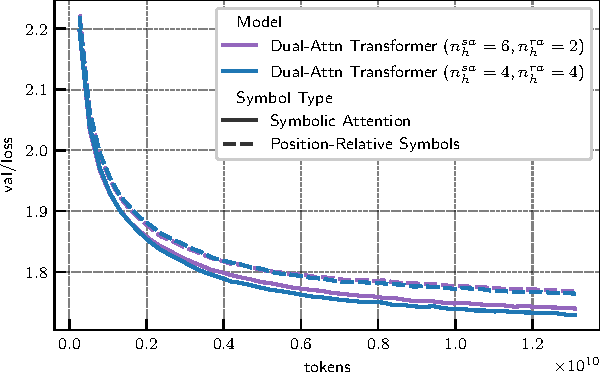
\includegraphics{figs/experiments/tiny_stories/d64L4_ablation_symboltype_asymra.pdf}
    \end{subfigure}
    \begin{subfigure}{0.45\textwidth}
        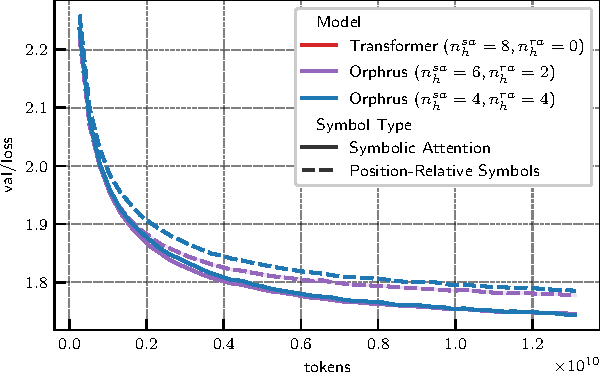
\includegraphics{figs/experiments/tiny_stories/d64L4_ablation_symboltype_symra.pdf}
    \end{subfigure}
\end{figure}

% add figure with d=128, L=4, 6